\documentclass{article}
\usepackage{amsmath}
\usepackage{graphicx}

\begin{document}

\title{Chapter 2}
\author{Amarnath Patel}
\date{\today}

\maketitle

\section{2-1}

We can describe objects in an idealized manner in the representation of a `particle'
To describe the motion of a particle, we need to describe the `position' of the particle and how position changes as the particle moves.
The change in something can be called displacement, so $x_f - x_i = \Delta x$. Average speed is equal to $\frac{total \space distance}{total \space time}$ = $\frac{s}{\Delta t}$.
Velocity is speed and direction and the `average velocity' is represented as $v_{av \, x}$ = $\frac{\Delta x}{\Delta t}$ = $\frac{x_f - x_i}{t_f - t_i}$ so $\Delta x = v_{av \, x} \Delta t$.
The next part is about slope but like everyone knows what slope is.

The instantaneous velocity $v_x$ is the limit of the ratio $\Delta x / \Delta t$ as $\Delta t$ approaches 0.
$v_x(t) = \lim_{\Delta t \to 0} \frac{\Delta x}{\Delta t}$

This is literally just a derivative of $dx/dt$. This is instantaneous velocity.

\section{2-2}

Acceleration is the rate of change of velocity with respect to time. The average acceleration, $a_{av \, x}$ for a particular interval $\Delta t$ is defined as the change in velocity $\Delta v$ divided by that time interval.
$a_{av \, x} = \frac{\Delta v_x}{\Delta t} = \frac{v_{fx} - v_{ix}}{t_f - t_i}$
Instanenous acceleration is the limit of the ratio $\Delta v_x$ / $\Delta t$ as $\Delta t$ approaches 0.
Acceleration therefore is the derivative of velocity $v_x$ with respect to time $dv_x / dt$. Velocity is the derivative of the position x with respect to t, acceleration is the second derivative of x with respect to t, $d^2x / dt^2$. 
When $v_x$ and $a_x$ are both positive and becoming more positive the speed is increasing. If they are both negative, and $v_x$ is becoming more negative the speed is again increasing. When they have oppposite signs the object is slowing down. If velocity is positive and acceleartion is negative and velocity is positive but becoming less positive the speed is decreasing. If velocity is negative and acceleration is positive and velocity is becoming less negative the speed is again decreasing. Basically, if they have the same sign the speed is increasing, if opposite the speed is decreasing.

\begin{figure}[h]
    \centering
    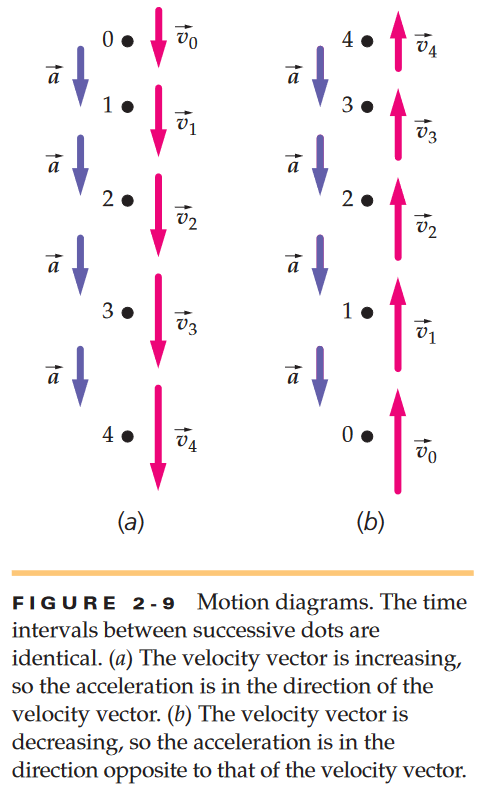
\includegraphics[width=1\textwidth]{assets/1.png}
    \caption{Motion Diagrams}
    \label{fig:my_label}
\end{figure}


\section{2-3}

If a particle has constant acceleration that means that the average acceleration is equal to its acceleration.
\end{document}